\chap{Operational Amplifier - OPAMP}
\section{Introduction}
Operational Amplifiers, also known as Op-amps, are basically a voltage amplifying device designed to be used with components like capacitors and resistors, between its in/out terminals. They are essentially a core part of analog devices. Feedback components like these are used to determine the operation of the amplifier. The amplifier can perform many different operations, giving it the name Operational Amplifier.\\

One key to the usefulness of these little circuits is in the engineering principle of feedback, particularly negative feedback, which constitutes the foundation of almost all automatic control processes. The principles presented in this section, extend well beyond the immediate scope of electronics. It is well worth the electronics student’s time to learn these principles and learn them well.\\

Operational amplifiers can have either a closed-loop operation or an open-loop operation. The operation (closed-loop or open-loop) is determined by whether or not feedback is used. Without feedback the operational amplifier has an open-loop operation. This open-loop operation is practical only when the operational amplifier is used as a cooperator (a circuit which compares two input signals or compares an input signal to some fixed level of voltage). As an amplifier, the open-loop operation is not practical because the very high gain of the operational amplifier creates poor stability. (Noise and other unwanted signals are amplified so much in open-loop operation that the operational amplifier is usually not used in this way.) Therefore, most operational amplifiers are used with feedback (closed-loop operation).

\newpage
\section{Closed Loop Operation}

Operational amplifiers are used with degenerative (or negative) feedback which reduces the gain of the operational amplifier but greatly increases the stability of the circuit. In the closed-loop configuration, the output signal is applied back to one of the input terminals. This feedback is always degenerative (negative). In other words, the feedback signal always opposes the effects of the original input signal. One result of degenerative feedback is that the inverting and non-inverting inputs to the operational amplifier will be kept at the same potential.\\

Closed-loop circuits can be of the inverting configuration or non-inverting configuration.\\

\subsection{Non inverting configuration}

The typical circuit for this configuration is shown in the figure bellow:
\begin{figure}[!htp]
    \centering
    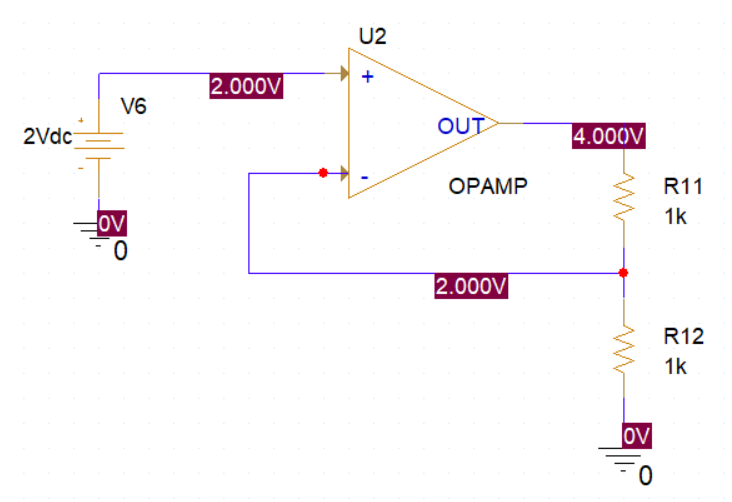
\includegraphics[width = 4in]{source/picture/bai_5/opam1.PNG}
    \caption{Non inverting configuration}
    \label{lab05_manual1}
\end{figure}

The new component, named also OPAMP (Operational Amplifier) is easily found in the favorite list of the PSPICE.\\

In order to explain the 4V at the ouput, it is obviously that $V(+) = V(-) = 2V$ in a closed loop configuration. Therefore, from a resistor bridge at the output, $V_{OUT} = 4V$.

\subsection{Inverting configuration} In this configuration, the output is connected directly to a pin of the opamp as follow:
\newpage
\begin{figure}[!htp]
    \centering
    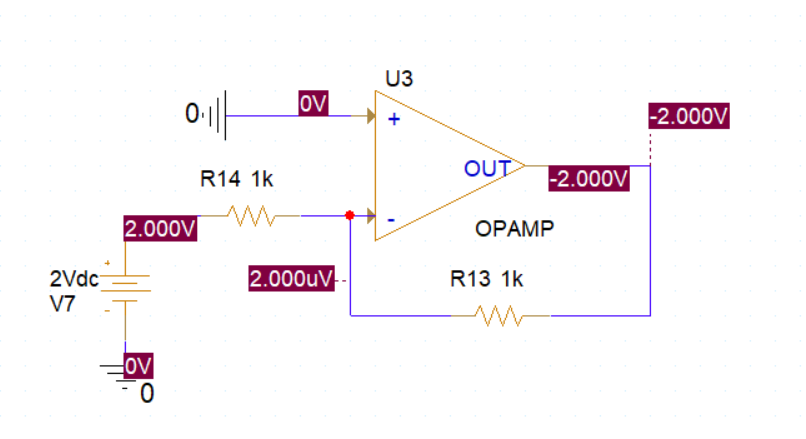
\includegraphics[width = 4.5in]{source/picture/bai_5/opam2.PNG}
    \caption{Inverting configuration}
    \label{lab05_manual2}
\end{figure}
As the output voltage is negative, which is inverted to the input, the name of this circuit is the invert connection. Students are proposed to perform calculations to confirm the output, which is $-2V$.\\



\section{Exercise and Report}
\subsection{Voltage Follower}
Voltage follower is one of the simplest uses of an operational amplifier, where the output voltage is exactly same as the input voltage applied to the circuit. In other words, the gain of a voltage follower circuit is unity. The connections are proposed as follows:


\begin{figure}[!htp]
    \centering
    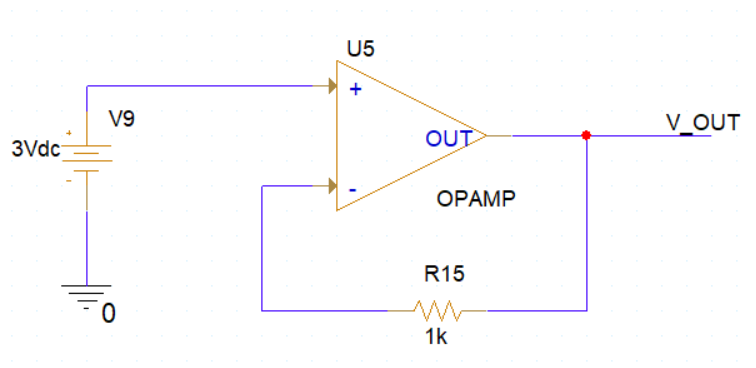
\includegraphics[width = 4.5in]{source/picture/bai_5/opam_follower.PNG}
    \caption{Opamp follower circuit}
    \label{lab05_opamp_follower}
\end{figure}

A voltage follower has low output impedance and extremely high input impedance, and this makes it a simple and effective solution to problematic impedance relationships. If a high-output-impedance sub-circuit must transfer a signal to a low-input-impedance sub-circuit, a voltage follower placed between these two sub-circuits will ensure that the full voltage is delivered to the load.\\

\textbf{Students are propose to run the simulation with bias mode to confirm that $V_{OUT} = V(+)$. The feedback resistance is also required to change.\\}

Your calculations are presented here to prove $V_{OUT} = V(+)$ with any value of R15. 

% https://www.allaboutcircuits.com/video-tutorials/op-amp-applications-voltage-follower/

% \subsection{High-Current Voltage Follower}

% https://www.allaboutcircuits.com/technical-articles/how-to-buffer-an-op-amp-output-for-higher-current-part-1/

\subsection{High-Current Voltage Follower}
The voltage follower’s low output impedance makes it a good circuit for driving current into a low-impedance load, but it’s important to remember that most op-amps are not designed to deliver large output currents. The most basic circuit for buffering an op-amp’s output current is the following:

\begin{figure}[!htp]
    \centering
    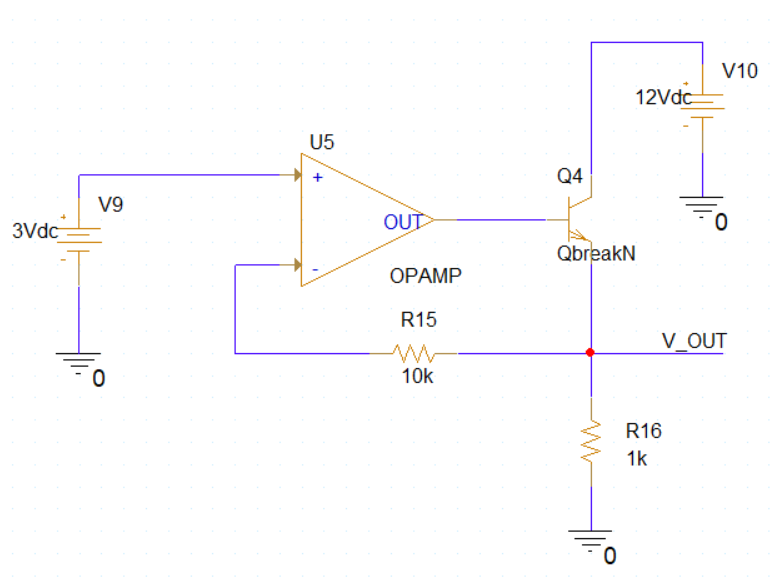
\includegraphics[width = 4.5in]{source/picture/bai_5/opam_follower_2.PNG}
    \caption{Opamp follower circuit}
    \label{lab05_opamp_follower_2}
\end{figure}

The voltage at the positive pin of the Opamp is copied to $V_{OUT}$. In this schematic, R16 is used to simulate a load device, which can be a motor or an high power LED. However, in this case, there is a high current can pass the load. \\

Students are proposed to run the simulation with bias configuration, capture the results and place them in the report. \\

Finally, your computations go here to explain the results. 

\subsection{Voltage Follower with Gain}
This basic circuit is not limited to the unity-gain configuration. As with a non-buffered op-amp, you can insert resistors into the feedback path to create overall gain from the input to the load voltage. Here is the non-unity-gain version of the circuit:

\begin{figure}[!htp]
    \centering
    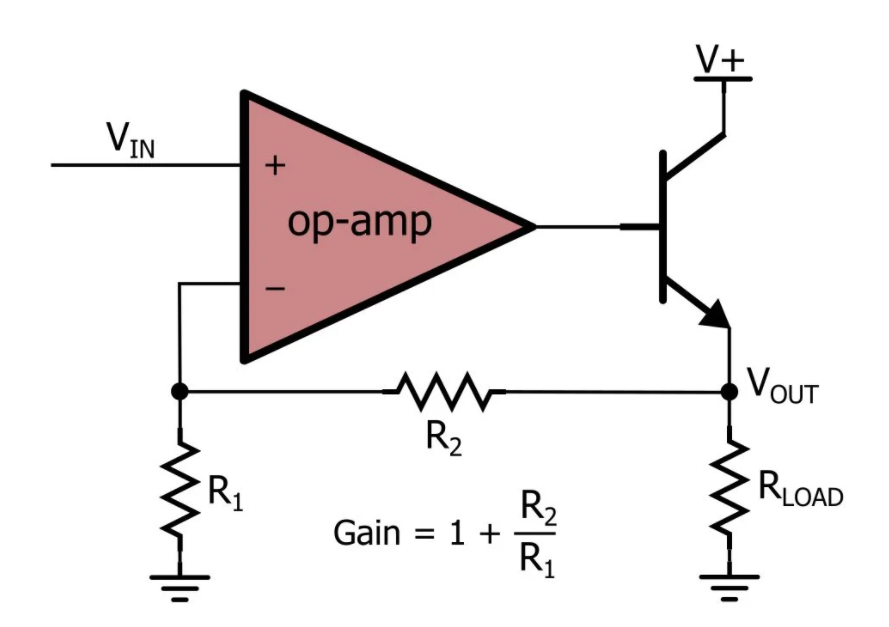
\includegraphics[width = 4in]{source/picture/bai_5/opam_follower_3.PNG}
    \caption{Opamp follower with gain for the output}
    \label{lab05_opamp_follower_3}
\end{figure}

Students are proposed to implement this circuit on PSPICE with input is 2V and the gain is 3. The voltage supply for the load side is 12VDC. Value of $R_{LOAD}$ is 1K. \\

The simulation results in PSPICE (bias configuration) are presented here. Moreover, a short explanations are required in this report to explain the gain of the output follower voltage. 


\subsection{Summing Amplifier}

Students are proposed to implement following schematic in PSPICE and run the simulation with R1 = 1K, R2 = 2K, R3 = 5K, Rf = 9K, Ri = 1K. There inputs are V1 = 1V, V2 = 2V and V3 = 3V. This circuit is a non inverting summing configuration using opamp.

\begin{figure}[!htp]
    \centering
    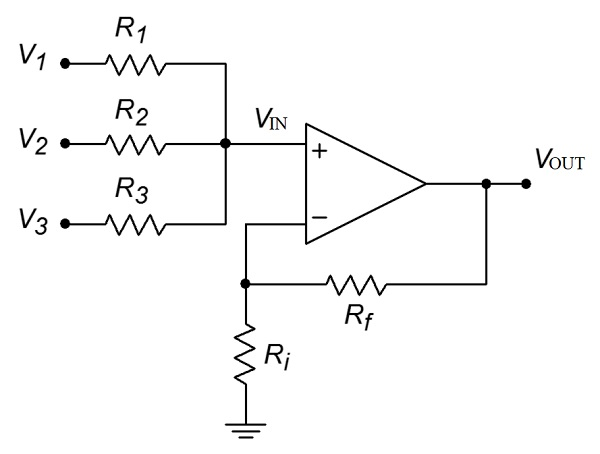
\includegraphics[width = 4in]{source/picture/bai_5/Non_Inv_Sum.jpg}
    \caption{Non inverse summing using OPAMP}
    \label{lab05_opamp_non_inv_sum}
\end{figure}

Students are proposed to design the schematic and place the results in this report.\\

\textbf{\textit{Your image goes here}}

Your calculations go here to explain the value of $V_{OUT}$

The second type of the summing amplifier is proposed as follows:
\begin{figure}[!htp]
    \centering
    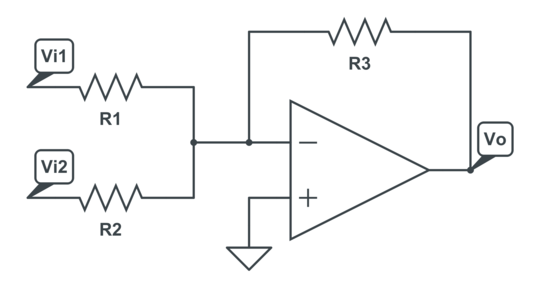
\includegraphics[width = 4in]{source/picture/bai_5/inv_sum.png}
    \caption{Inverse summing using OPAMP}
    \label{lab05_opamp_non_inv_sum}
\end{figure}

Students are proposed to do the same steps above, with R1 = 1K, R2 = 2K, R3 = 10K and V1 = 1V, V2 = 5V.

\subsection{Low Pass Filter}
% https://www.allaboutcircuits.com/video-tutorials/op-amps-low-pass-and-high-pass-active-filters/
Low pass filter is a filter which passes all frequencies from 0Hz (DC current) to upper cut-off frequency $f_H$ and rejects any signals above this frequency. A picture to demonstrate a low pass filter behavior is shown in the figure bellow:

\begin{figure}[!htp]
    \centering
    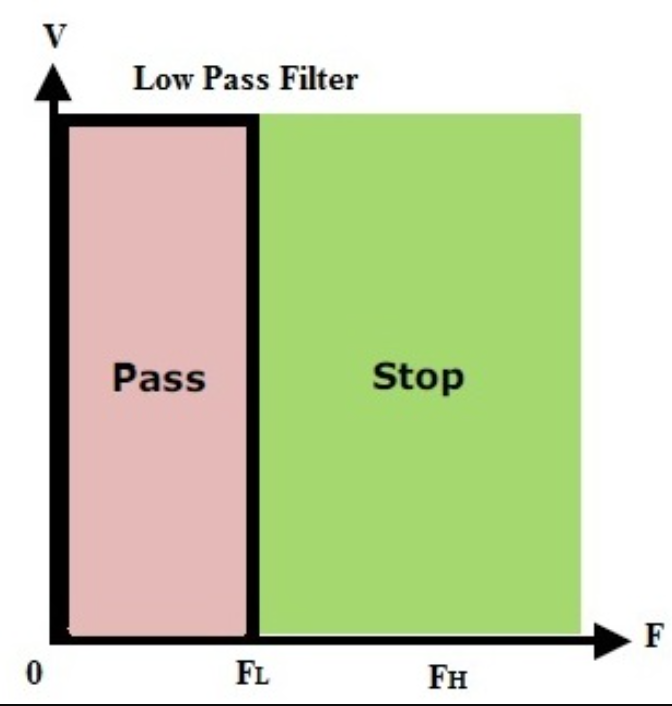
\includegraphics[width = 2.5in]{source/picture/bai_5/low_filter1.PNG}
    \caption{Low pass filter principles}
    \label{lab05_low_filter1}
\end{figure}

Similar to the closed loop configuration, there also 2 types of low pass filter, including the inverting and non-inverting low pass filter. The figure bellow is an inverting low pass filter.

\begin{figure}[!htp]
    \centering
    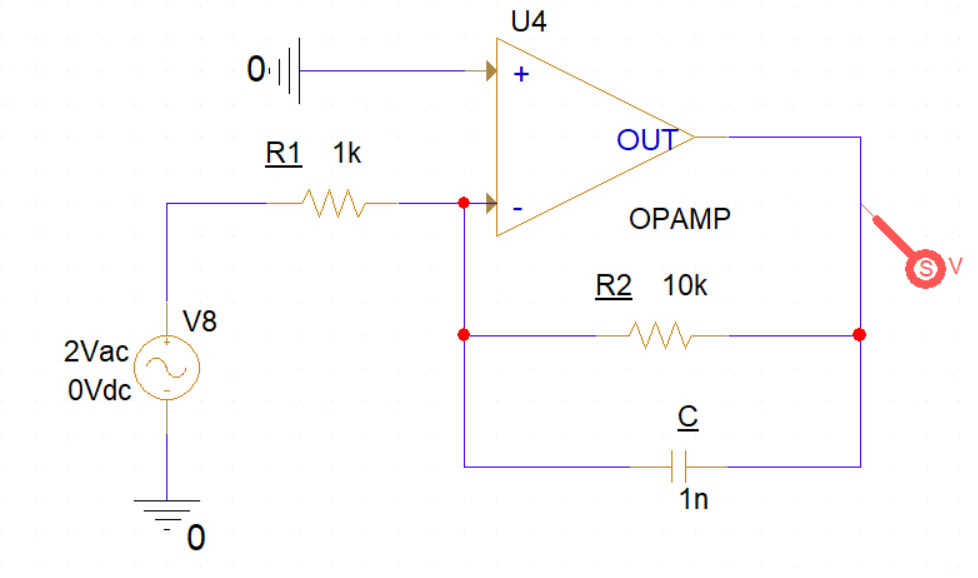
\includegraphics[width = 4in]{source/picture/bai_5/low_filter2.PNG}
    \caption{Inverting low pass filter}
    \label{lab05_low_filter2}
\end{figure}

The cut-off frequency is determined by this equation:
\begin{equation*}
    f_H = \frac{1}{2\pi R_2 C}
\end{equation*}

By applying the value of $R2 = 10KOhm$ and $C=1nF$, the cut-off frequency is around $16KHz$. In order to see the results, students are proposed to run the AC Sweep simulation profile (\textbf{Linear Type, Start and Stop frequency are 1Hz and 50kHz, 200 points}), as follows:

\begin{figure}[!htp]
    \centering
    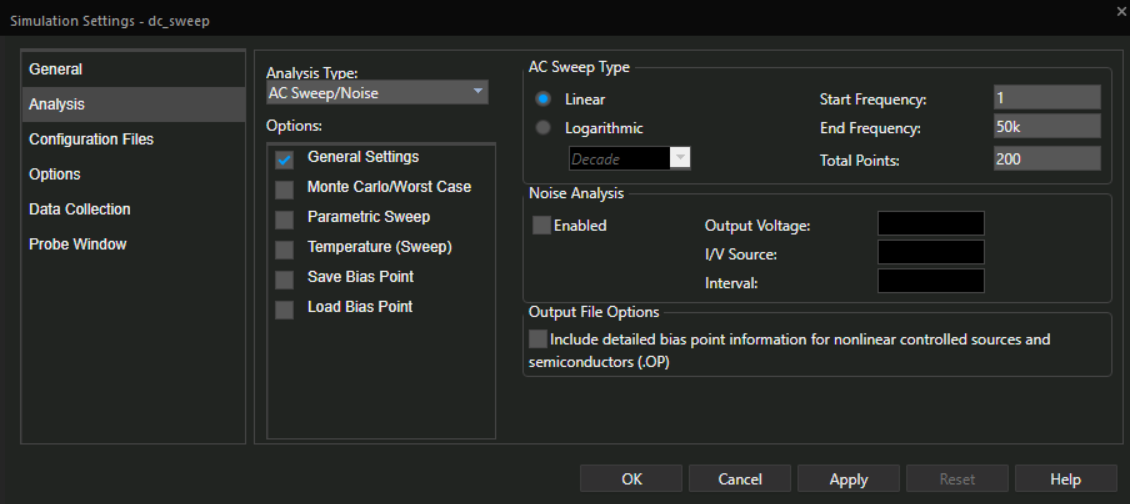
\includegraphics[width = 5in]{source/picture/bai_5/low_filter3.PNG}
    \caption{AC Sweep simulation profile}
    \label{lab05_low_filter3}
\end{figure}

The final results can be archived like the figure bellow:

\begin{figure}[!htp]
    \centering
    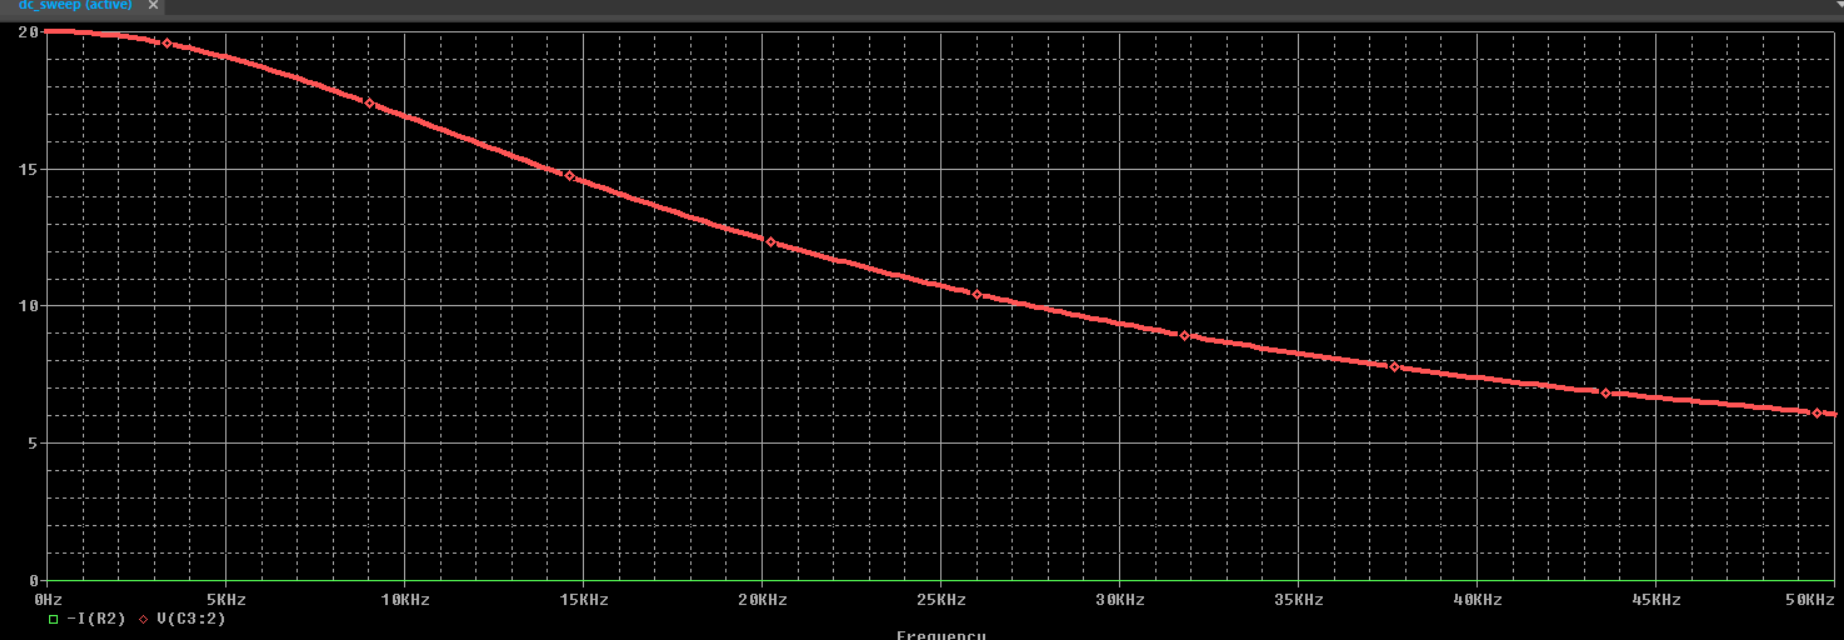
\includegraphics[width = 5in]{source/picture/bai_5/low_filter4.PNG}
    \caption{Simulation results}
    \label{lab05_low_filter4}
\end{figure}

\textbf{It is said that the cut-off frequency point having the gain reduced 3dB}. The gain at 0Hz is 10 (input voltage is 2V and output voltage is 20V), or $20log(10) = 20dB$, meanwhile, the gain at 16kHz is 7 (input voltage is 2V and output voltage is 14V), or $20log(7) = 16.9$. \\

The second type of a low pass filter, the non-inverting configuration, is presented as follows:

\begin{figure}[!htp]
    \centering
    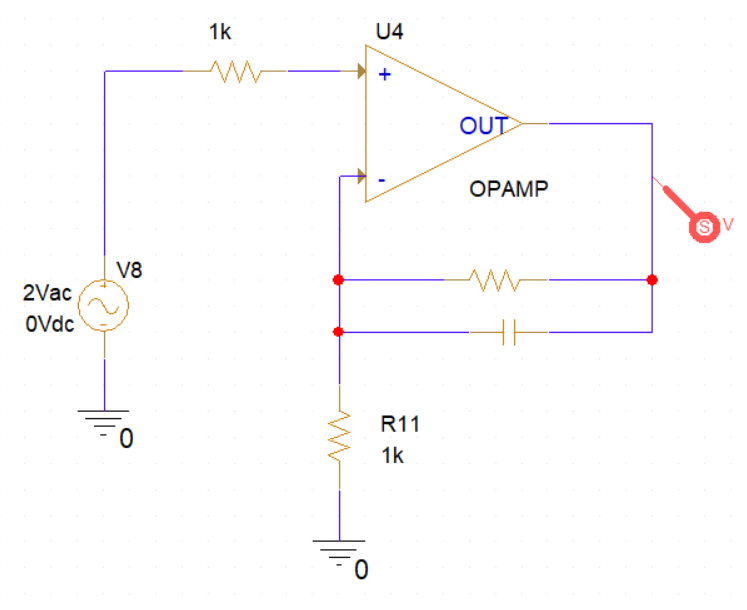
\includegraphics[width = 4in]{source/picture/bai_5/low_filter5.PNG}
    \caption{Non-inverting low pass filter}
    \label{lab05_low_filter5}
\end{figure}

\textbf{Students are proposed to calculate the value of R and C to have the amplifier factor equal to 10 and the cut-off frequency is the same as the previous example. The simulation result with AC Sweep mode is required to plot in this report as well.}

\subsection{High Pass Filter}
In contrast to the low pass filter, there is a high pass filter, which can be referred from this link:
\begin{center}
    \link{https://www.allaboutcircuits.com/video-tutorials/op-amps-low-pass-and-high-pass-active-filters/}
\end{center}

Students are proposed to implement a high pass filter in PSPICE and explain the behaviors of your high pass filter.

\subsection{Comparator with Hysteresis (Schmitt Trigger)}
% https://www.allaboutcircuits.com/tools/hysteresis-comparator-calculator/
The two resistors R1 and R2 act only as a "pure" attenuator (voltage divider). The input loop acts as a simple series voltage summer that adds a part of the output voltage in series to the circuit input voltage. This series positive feedback creates the needed hysteresis that is controlled by the proportion between the resistances of R1 and the whole resistance (R1 and R2). The effective voltage applied to the op-amp input is floating so the op-amp must have a differential input.\\

\begin{figure}[!htp]
    \centering
    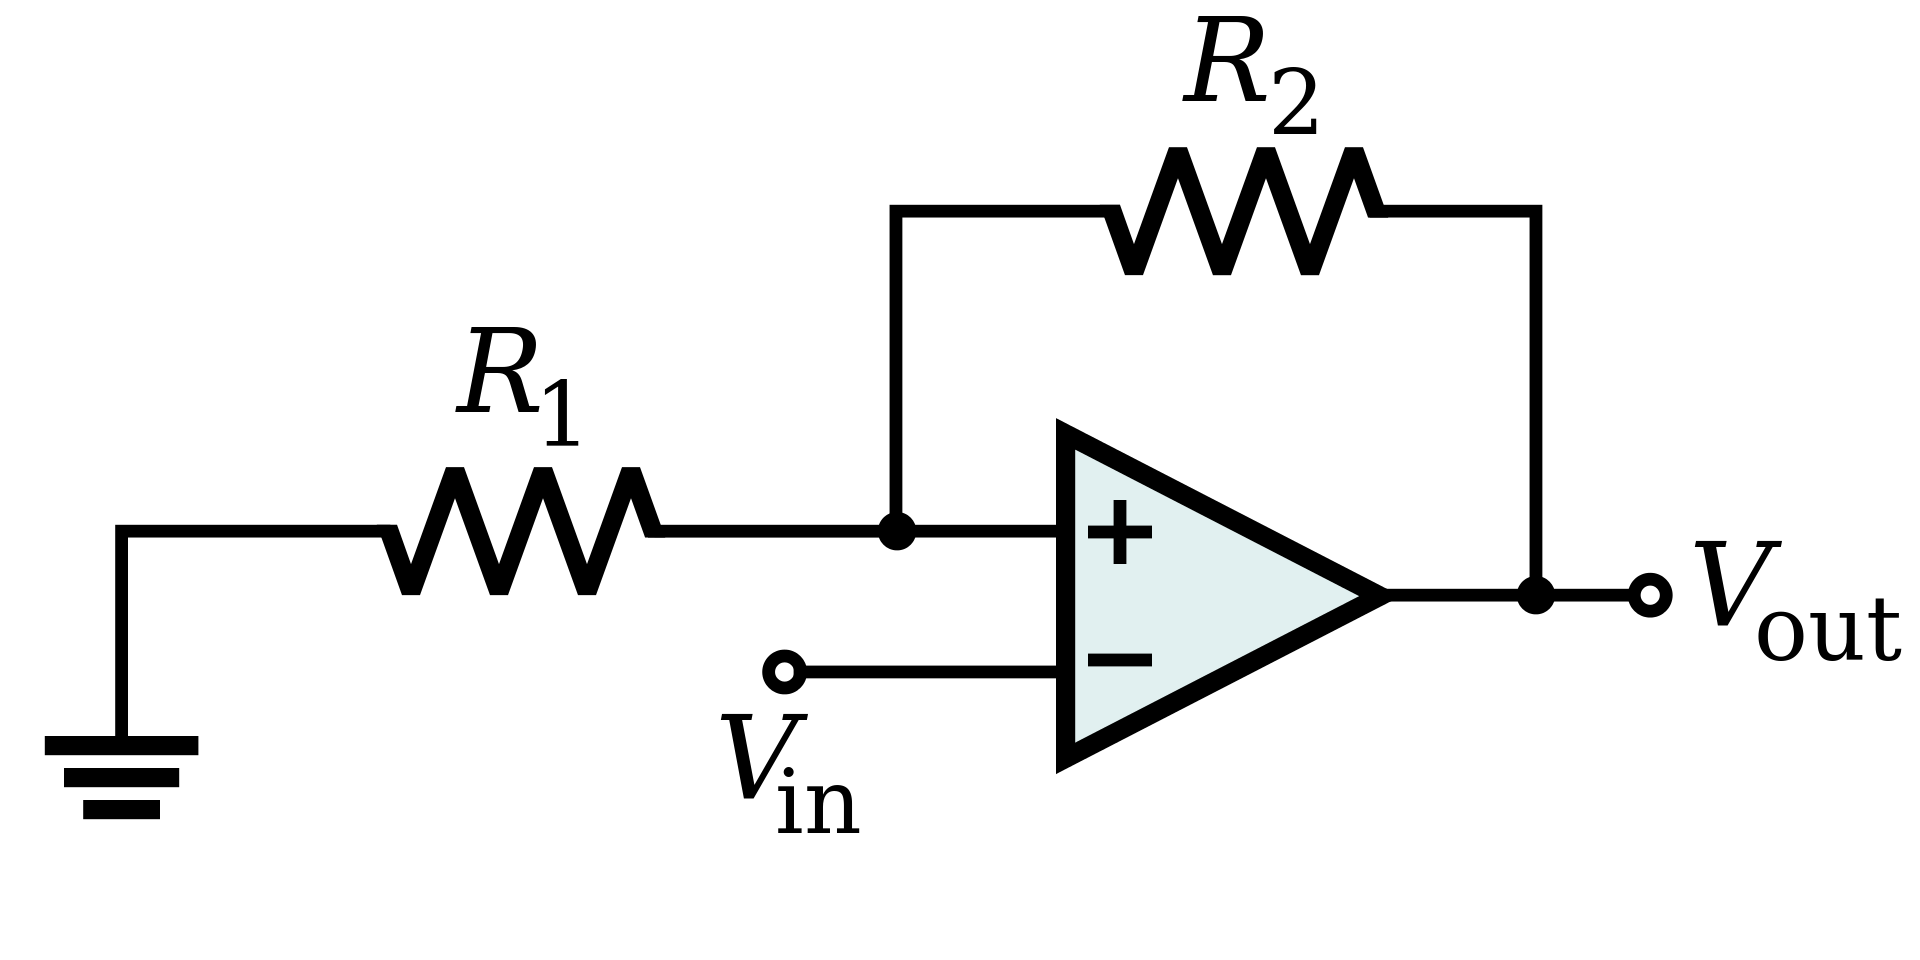
\includegraphics[width = 4in]{source/picture/bai_5/sTrigger.png}
    \caption{Inverting Schmitt trigger}
    \label{lab05_low_filter5}
\end{figure}


The circuit is named inverting since the output voltage always has an opposite sign to the input voltage when it is out of the hysteresis cycle (when the input voltage is above the high threshold or below the low threshold). However, if the input voltage is within the hysteresis cycle (between the high and low thresholds), the circuit can be inverting as well as non-inverting. The output voltage is undefined and it depends on the last state so the circuit behaves like an elementary latch.\\

In PSPice, this trigger is implemented as follows, with 3 voltage markers:

\begin{figure}[!htp]
    \centering
    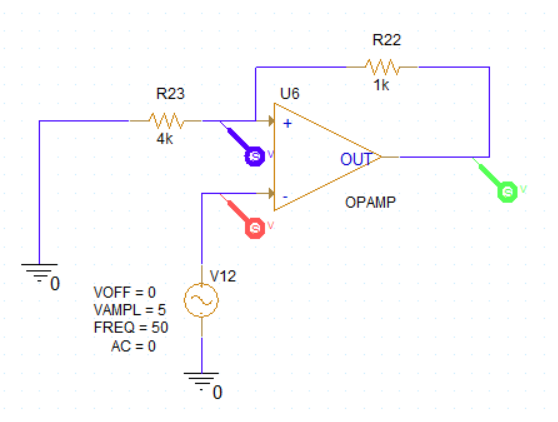
\includegraphics[width = 4in]{source/picture/bai_5/sTrigger2.png}
    \caption{Schmitt trigger in PSPICE}
    \label{lab05_low_filter5}
\end{figure}

The OPAMP device is modified in the \textbf{Properties} windows (right click on the component and chose Edit Properties or double click on the component), in order to set the VPOS and VNEG to +5V and -5V, as follows:

\begin{figure}[!htp]
    \centering
    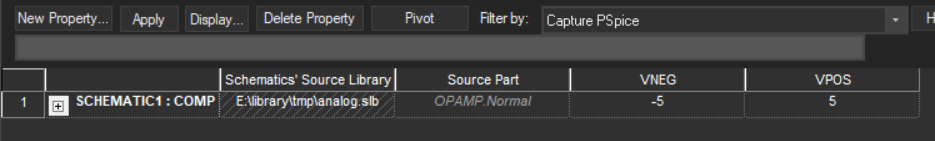
\includegraphics[width = 4in]{source/picture/bai_5/sTrigger4.png}
    \caption{Schmitt trigger in PSPICE}
    \label{lab05_low_filter5}
\end{figure}


The simulation profile in this exercise is the \textbf{Time Domain}, and is configured as follows:

\begin{figure}[!htp]
    \centering
    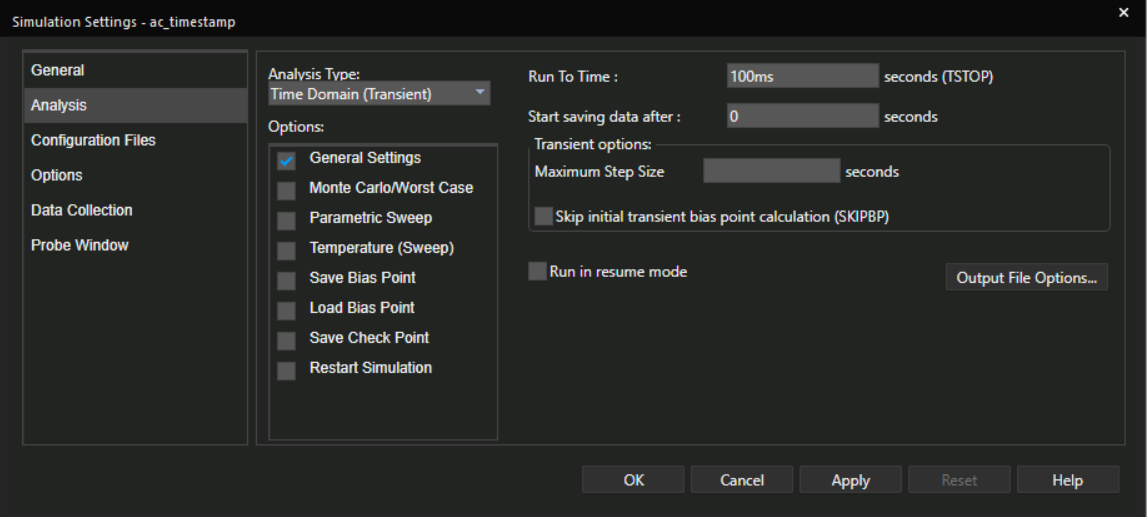
\includegraphics[width = 4in]{source/picture/bai_5/sTrigger3.png}
    \caption{Simulation profile}
    \label{lab05_low_filter5}
\end{figure}

Finally, the simulation results can be archived as follows:

\begin{figure}[!htp]
    \centering
    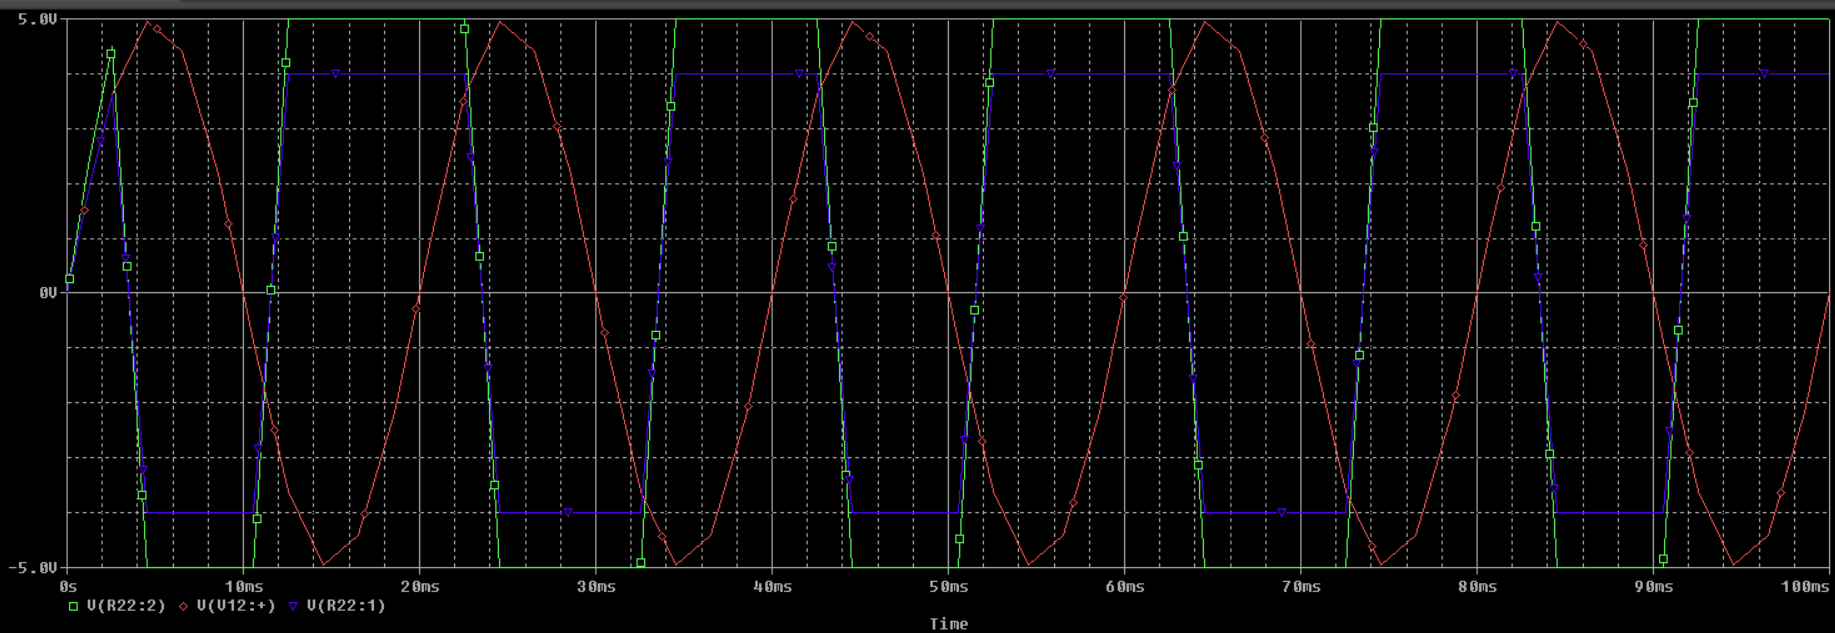
\includegraphics[width = 5.5in]{source/picture/bai_5/sTrigger5.png}
    \caption{Schmitt trigger simulation results}
    \label{lab05_low_filter5}
\end{figure}

\textbf{Students are proposed to explain the signal at the output of the opamp. Why the signal is toggled at +4V and -4V.}


\section{Altium Designer}
\subsection{LED Driver}
In this project, we will show how to build a simple LED driver circuit. A simple driver based on BJT is proposed in this section.

\subsubsection{Schematic design}
The manual for the schematic is posted in this link:

\begin{center}
    \link{https://www.youtube.com/watch?v=ftiX8peTsiw}
\end{center}

Students are proposed to design the schematic and place the results in this report.\\

\textbf{\textit{Your image goes here}}

\subsubsection{PCB layout}
The manual for PCB layout is posted in this link:\\

\begin{center}
    \link{https://www.youtube.com/watch?v=btpAoh3nmBU}
\end{center}

\textbf{\textit{Your image goes here}}

\subsection{Relay Controller}

\subsubsection{Schematic design}
The manual for the schematic is posted in this link:

\begin{center}
    \link{https://www.youtube.com/watch?v=VcO\_F97ydFM}
\end{center}

Students are proposed to design the schematic and place the results in this report.\\

\textbf{\textit{Your image goes here}}

\subsubsection{PCB layout}
The manual for PCB layout is posted in this link:\\

\begin{center}
    \link{https://www.youtube.com/watch?v=Dbqcb0zQ0E8}
\end{center}

\textbf{\textit{Your image goes here}}